% --------------------------------------------------------------
% This is all preamble stuff that you don't have to worry about.
% Head down to where it says "Start here"
% --------------------------------------------------------------
 
\documentclass[12pt]{article}
 
\usepackage[margin=1in]{geometry} 
\usepackage{amsmath,amsthm,amssymb}
 
\newcommand{\N}{\mathbb{N}}
\newcommand{\Z}{\mathbb{Z}}
 
\newenvironment{intro}[2][I Introduction]{\begin{trivlist}
\item[\hskip \labelsep {\bfseries #1}\hskip \labelsep {\bfseries #2}]}{\end{trivlist}}

\newenvironment{p1}[2][II Feature and Weak Classifier Design]{\begin{trivlist}
\item[\hskip \labelsep {\bfseries #1}\hskip \labelsep {\bfseries #2}]}{\end{trivlist}}

\newenvironment{p2}[2][III Adaboost for Classifier Selection]{\begin{trivlist}
\item[\hskip \labelsep {\bfseries #1}\hskip \labelsep {\bfseries #2}]}{\end{trivlist}}

\newenvironment{p3}[2][IV Realboost for Face Detection]{\begin{trivlist}
\item[\hskip \labelsep {\bfseries #1}\hskip \labelsep {\bfseries #2}]}{\end{trivlist}}

\usepackage{graphicx}
\graphicspath{{./}}

\begin{document}
 
% --------------------------------------------------------------
%                         Start here
% --------------------------------------------------------------
 
\title{Project II Detecting Faces in Images by Boosting Technique}
\author{Yunzhong He\\ %replace with your name
204010749} %if necessary, replace with your course title
 
\maketitle

\begin{intro}{}
\item{}
In this project, we trained around 50000 16X16 images with boosting technique for face detection. We designed ~2000 Harr-like features, and use each one of them as a weak classifier. We then trained Adaboost with 105 iterations and picked 105 weak classifiers among the 2000. Lastly, we trained the top 10, 50, 100 weak classifiers with RealBoost and obtained a strong classifier to detect faces from our class.
\end{intro}

\begin{p1}{}
\item{}
We designed Harr-like features with the following patterns, and each can be in different sizes and flipped color. Aligning them to different positions, we obtained around 2000 features.
\begin{center}
		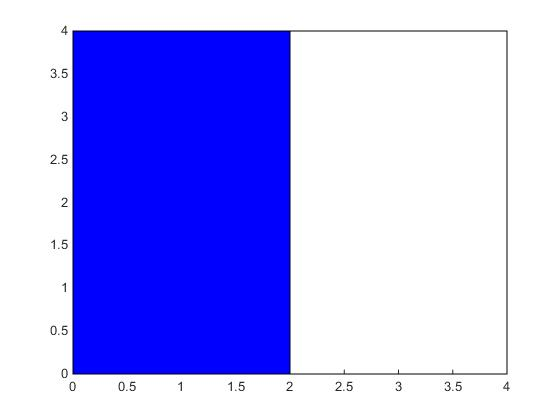
\includegraphics[height=2cm]{features/rec2_1.jpg}
		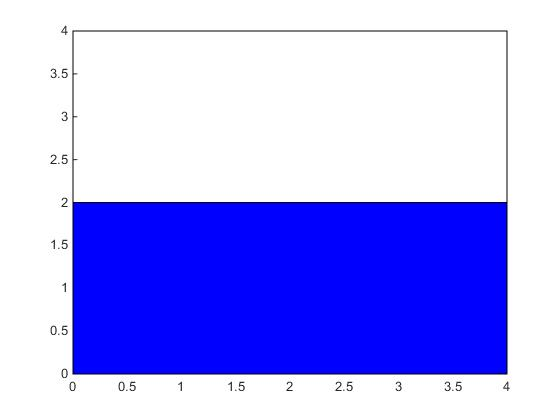
\includegraphics[height=2cm]{features/rec2_2.jpg}
		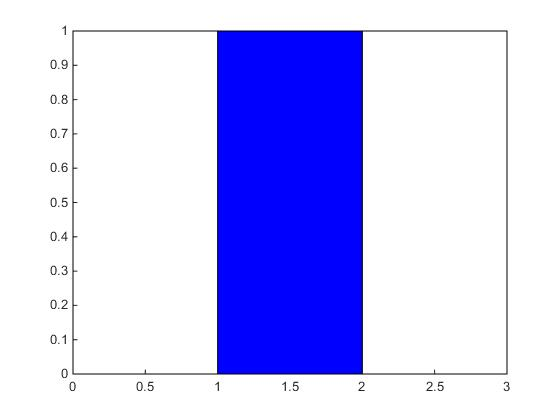
\includegraphics[height=2cm]{features/rec3_1.jpg}
\end{center}
\begin{center}
		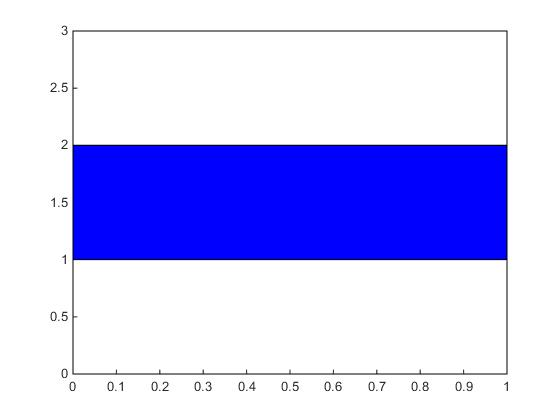
\includegraphics[height=2cm]{features/rec3_2.jpg}
		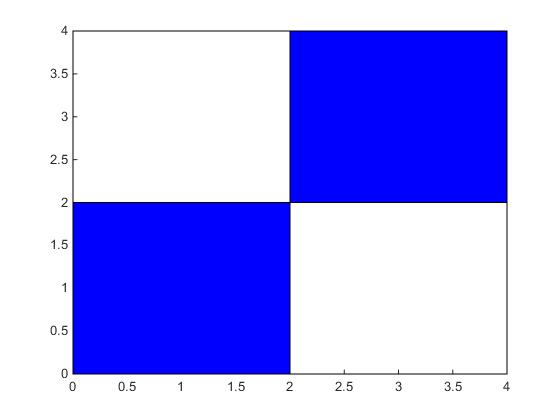
\includegraphics[height=2cm]{features/rec4_1.jpg}
		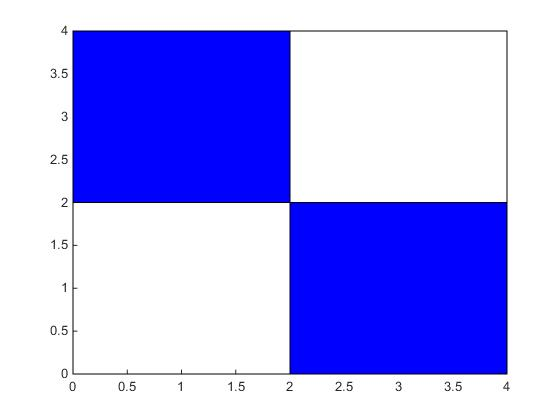
\includegraphics[height=2cm]{features/rec4_2.jpg}
\end{center}
\item{}
We therefore designed weak classifiers $h_1, h_2, ..., h_p$ such that each one projects the input image onto one of the features to obtain a real-valued result. And we trained them by first project all weighted training data into a vector, and move a threshold from left to right to find the one that minimizes weighted error.
\end{p1}

\begin{p2}{}
\item{III.1 Algorithm\\\\}
For Adaboost, the strong classifier is designed as follows
\begin{align*}
	F(x) = \alpha_1h_1(x) + \alpha_2h_2(x) + ... + \alpha_ph_p(x)
\end{align*}
At each iteration we choose the the classifer with minimal weighted error, and update the weighted error as follows
\begin{align*}
	D_t(X_i) = \frac{1}{Z_t}D_{t-1}(X_i)exp(-y_i\alpha_th_t(X_i))
\end{align*}
And it can be shown that choosing $\alpha_t = \frac{1}{2}log\frac{1-err_t(h_t)}{err_t(h_t)}$ gives the optimal result.
\item{III.2 Best Features\\\\}
After running Adaboost, we found the top 10 features with largest weights.
\begin{center}
		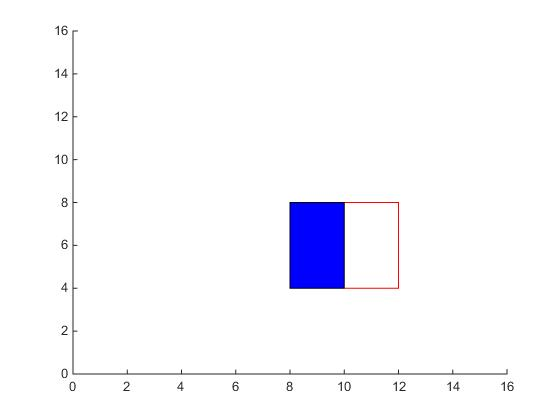
\includegraphics[height=2cm]{features/top1.jpg}
		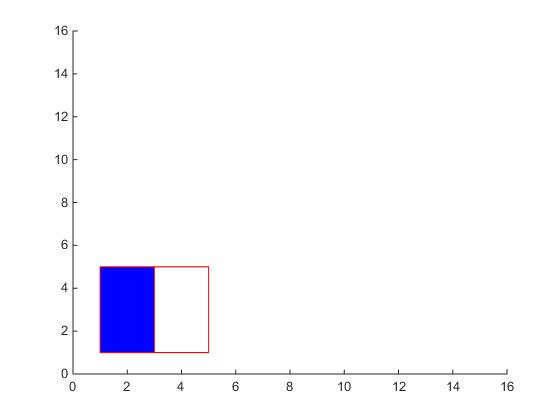
\includegraphics[height=2cm]{features/top2.jpg}
		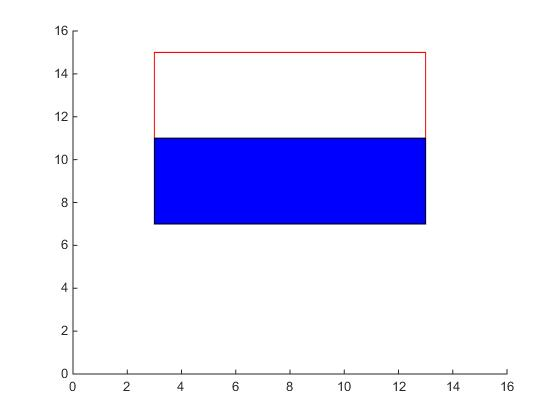
\includegraphics[height=2cm]{features/top3.jpg}
		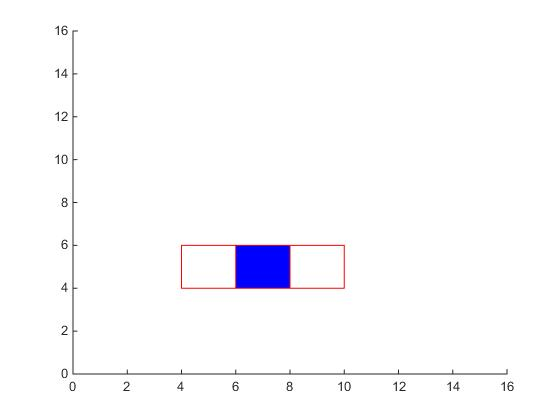
\includegraphics[height=2cm]{features/top4.jpg}
		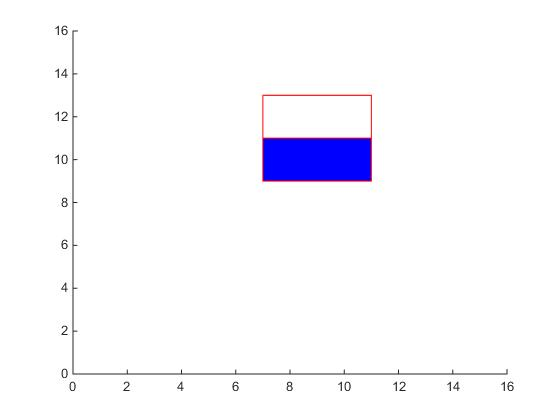
\includegraphics[height=2cm]{features/top5.jpg}
\end{center}
\begin{center}
		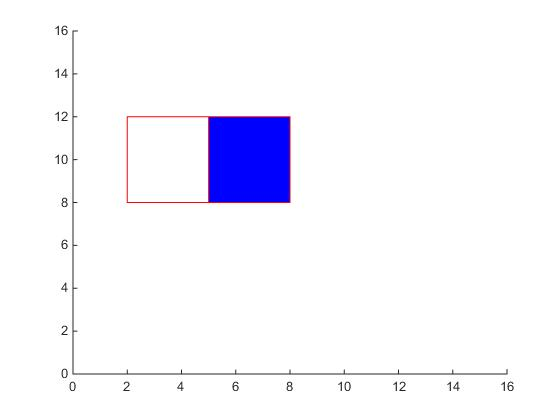
\includegraphics[height=2cm]{features/top6.jpg}
		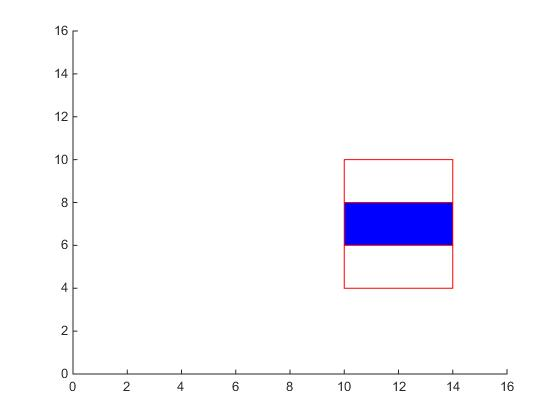
\includegraphics[height=2cm]{features/top7.jpg}
		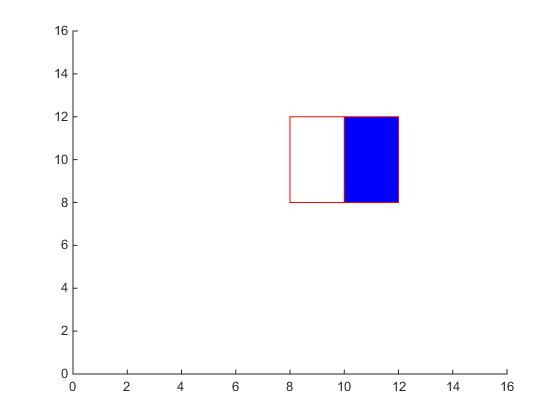
\includegraphics[height=2cm]{features/top8.jpg}
		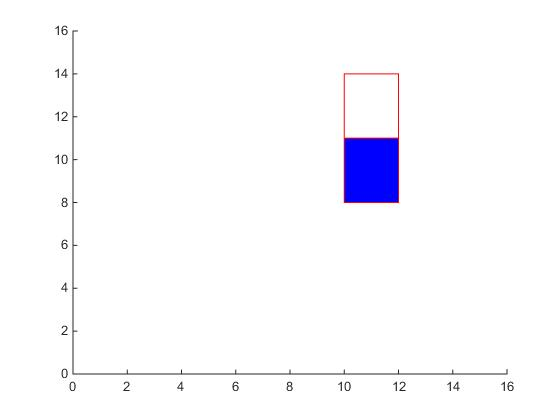
\includegraphics[height=2cm]{features/top9.jpg}
		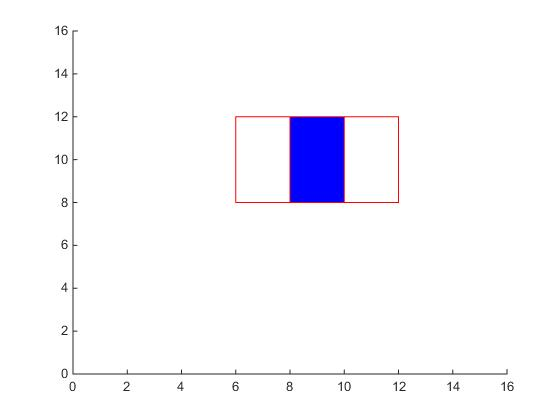
\includegraphics[height=2cm]{features/top10.jpg}
\end{center}
\item{III.3 Error Curves\\\\}
Below are the error curves at iteration 0, 10, 50 and 100 respectively. Notice that to speed up the training, I pruned some uninformative features (features where data points are clustered very closely) in the beginning, so the curves below show only the top informative features.
\begin{center}
		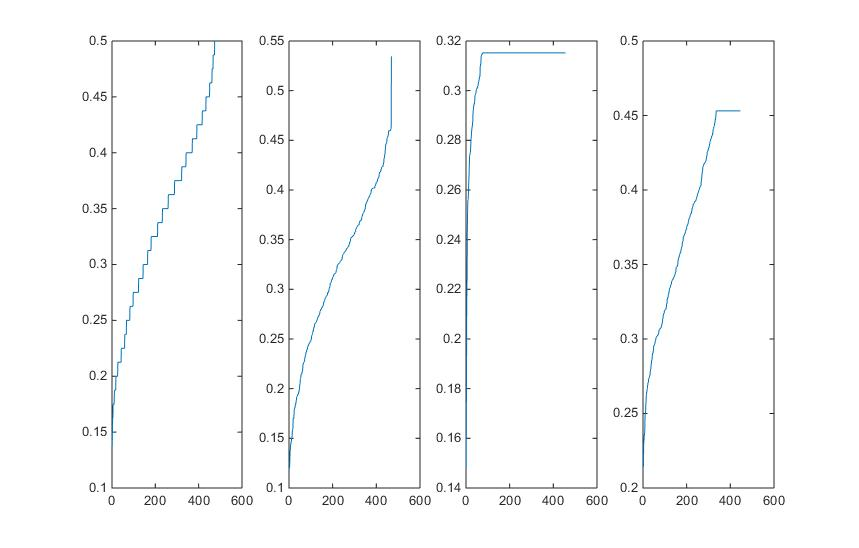
\includegraphics[height=10cm]{data/error_curve.jpg}
\end{center}
From the error curve we can see that initially many unpruned features have pretty good error rate, though some of the are still close to 0.5. Then the curve begins to shrink and eventually, some features's error rates are fixed at around 0.45, meaning they are no longer very useful.

\item{III.4 Histogram\\\\}
Below are histograms of all images on F(x) at iteration 10, 50 and 100 respectively.
\begin{center}
		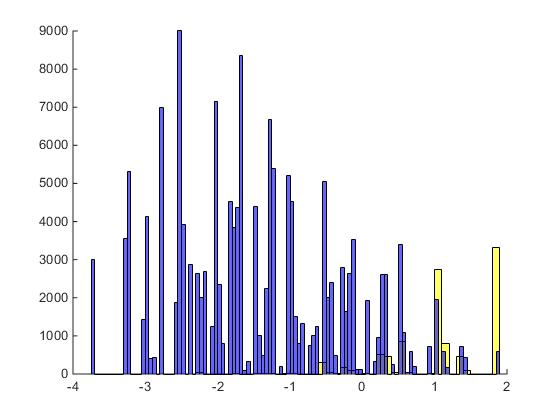
\includegraphics[height=4cm]{data/histogram_10.jpg}
		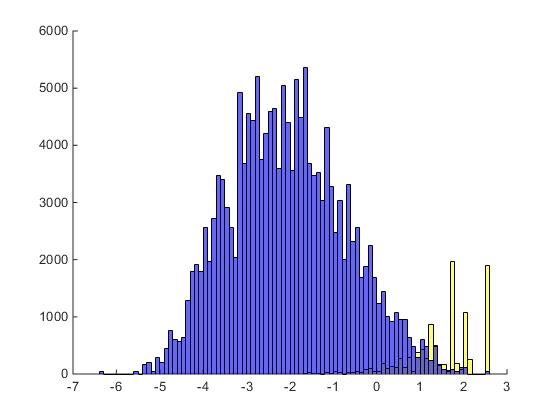
\includegraphics[height=4cm]{data/histogram_50.jpg}
		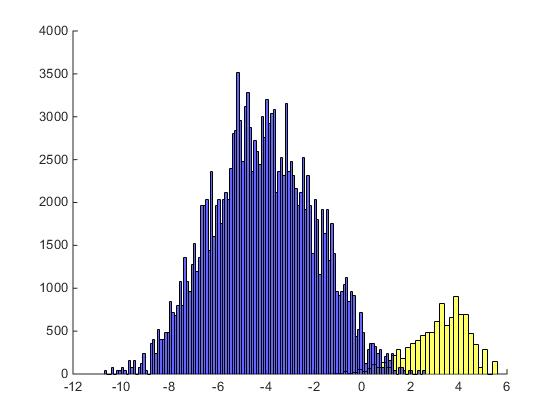
\includegraphics[height=4cm]{data/histogram_100.jpg}
\end{center}
From the histogram we can see that faces are gradually moving towards the right, whereas nonfaces are moving towards the left. And eventually they are well separated by x = 0.
\begin{center}
		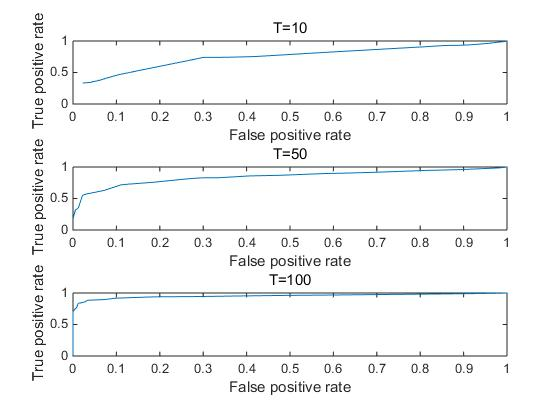
\includegraphics[height=10cm]{data/roc.jpg}
\end{center}
From the ROC curves above we can see that Adaboost is actually converging.
\end{p2}{}

\begin{p3}{}
\item{IV.1 Algorithm\\\\}
For realboost, we change the strong classifer design to the following
\begin{align*}
	F(x) = h_1(x) + h_2(x) + ... + h_p(x)
\end{align*}
where each $h_t$ is a weak classifier that we try to learn, and they are estimated by a vector of 100 bins $h_t = [h_{t, 1}, h_{t, 2}, ..., h_{t, 100}]$. It can be shown that letting
\begin{align*}
	h_{t, b} = \frac{1}{2}log\frac{p_t(b)}{q_t(b)}
\end{align*}
and choosing the $h_t$ that minimizes
\begin{align*}
	Z = 2\sum_{b=1}^B\sqrt{(p_t(b)q_t(b)}
\end{align*}
gives us the optimal $h_t$ at each iteration, where $p_t(b)$, $p_t(b)$ represents the number faces and nonfaces of the projected value onto a feature within the bth bin.

\item{IV.2 Error Curves\\\\}
At iteration 0, 10, 50 and 100 of the training process, we obtained the following error curves for unselected classifiers
\begin{center}
		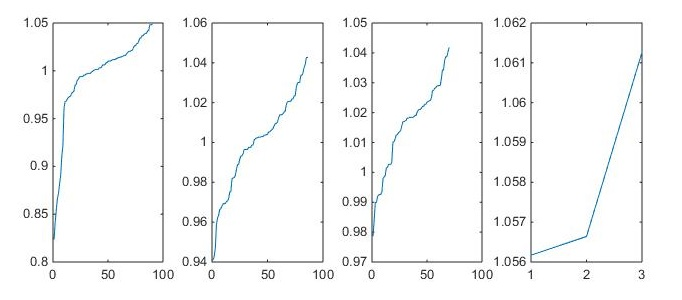
\includegraphics[height=7cm]{data/realboost_error_curve.jpg}
\end{center}
From the curves above we can see how $Z$ value is being adjusted. And towards the end only a few features with high weighted $Z$ values remaining.
\item{IV.3 Histograms\\\\}
Below are histograms of all images on F(x) at iteration 10, 50 and 100 respectively.
\begin{center}
		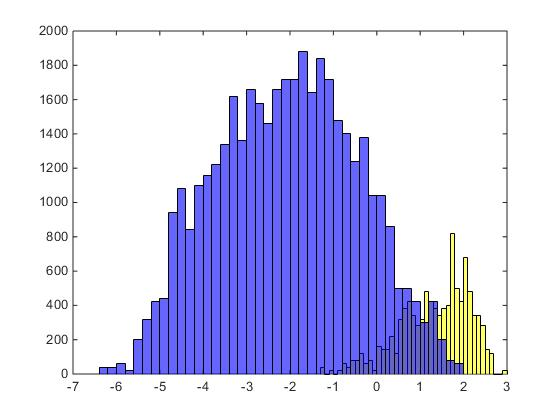
\includegraphics[height=4cm]{data/realboost_hist_10.jpg}
		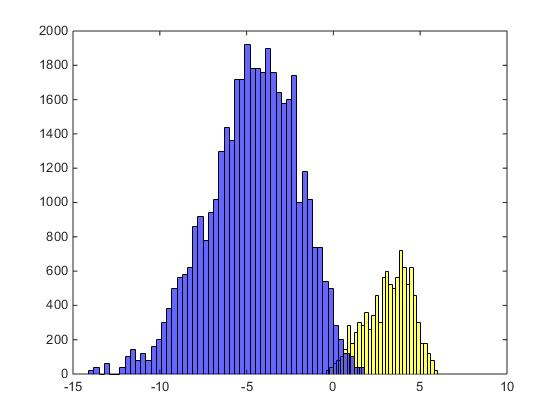
\includegraphics[height=4cm]{data/realboost_hist_50.jpg}
		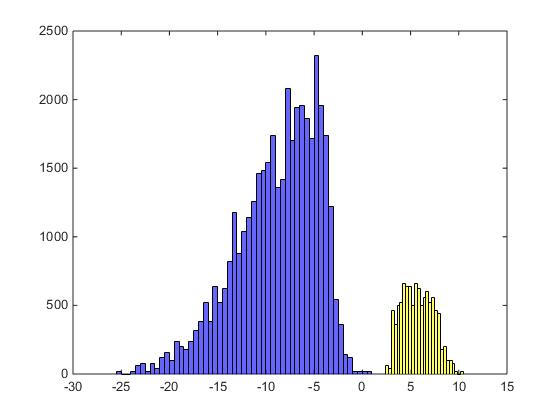
\includegraphics[height=4cm]{data/realboost_hist_100.jpg}
\end{center}
Comparing to the histograms in III, realboost seems to separate data better than adaboost at the same iteration, though we have a smaller feature pool this time. This may due to the fact that realboost allows more freedom in the learning of $F(x)$, and the choice of more informative features.
\item{IV.3 ROC Curves\\\\}
For histograms of iteration 10, 50 and 100 above, below are their corresponding ROC curves.
\begin{center}
		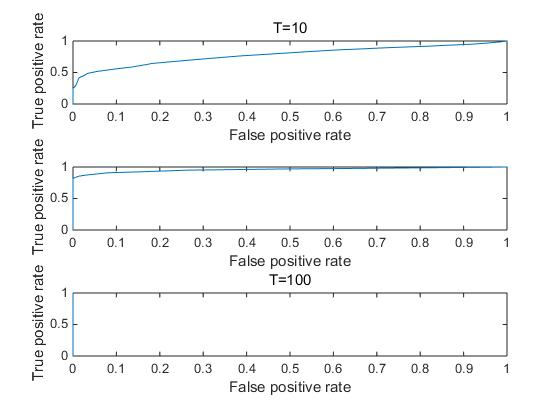
\includegraphics[height=10cm]{data/realboost_roc.jpg}
\end{center}
The ROC curves confirm with the results in histograms. And at the 100 iteration, we can see that the ROC curve is almost like a straignt line, meaning all training data are correctly classified.

\item{IV.4 Hard Negative Mining, Non-Maximum Supression and Window Size Tuning\\\\}
To avoid false positives, we manually added windows of the background image of the classroom as the nonface trainin set. \\
To achieve good results, we also turned the window size and the sliding window step size a bit. And eventually with window size 10, 12, 16, 20 and 32, the following result is achieved.
\begin{center}
		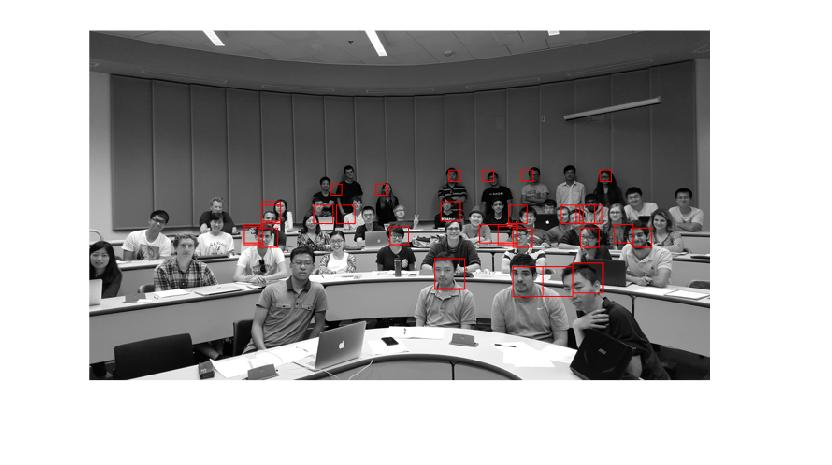
\includegraphics[height=10cm]{data/final.jpg}
\end{center}
From the image we can see that around 13 faces are correctly detected, with 6 false alarms, and 3 out of the 6 are close to sholders, while others make no sense at all.
\end{p3}{}

% --------------------------------------------------------------
%     You don't have to mess with anything below this line.
% --------------------------------------------------------------
 
\end{document}
